\documentclass{beamer}
\usetheme{Madrid}
\usecolortheme{default}

% Additional packages
\usepackage{graphicx}
\usepackage{amsmath}
\usepackage{listings}
\usepackage{xcolor}
\usepackage{subcaption}

% Custom colors and styles
\definecolor{codegreen}{rgb}{0,0.6,0}
\definecolor{codegray}{rgb}{0.5,0.5,0.5}
\definecolor{backcolour}{rgb}{0.95,0.95,0.92}

\lstdefinestyle{mystyle}{
    backgroundcolor=\color{backcolour},   
    commentstyle=\color{codegreen},
    basicstyle=\ttfamily\small,
    breakatwhitespace=false,         
    breaklines=true,                 
    keepspaces=true,                 
    showspaces=false,                
    showstringspaces=false,
    showtabs=false,                  
    tabsize=2
}
\lstset{style=mystyle}

\title{Neural Implicit Functions (NIF)}
\subtitle{Implementation and Analysis}
\author{Christian Beneke}
\date{10.02.2025}

\begin{document}

\begin{frame}
    \titlepage
\end{frame}

\begin{frame}{Outline}
    \tableofcontents
\end{frame}

\section{Introduction}
\begin{frame}{Problem Space \& Motivation}
    \begin{itemize}
        \item Spatio-temporal data modeled by PDEs is computationally challenging
        \item Current reduction methods (SVD, CAE) fail with:
        \begin{itemize}
            \item Variable geometry
            \item Adaptive meshing
        \end{itemize}
        \item Need for a scalable, mesh-agnostic approach
        \item Real-time engineering applications require efficient solutions
    \end{itemize}
\end{frame}

\section{Neural Implicit Functions - Theory}
\begin{frame}{Core Concept}
    \begin{itemize}
        \item NIFs represent continuous functions through neural networks
        \item Combines two neural networks:
        \begin{itemize}
            \item \textbf{ShapeNet:} Encodes spatial complexity
            \item \textbf{ParameterNet:} Models temporal/parametric dependencies
        \end{itemize}
        \item Mesh-agnostic representation
        \item Continuous output for any input coordinate
    \end{itemize}
\end{frame}

\section{Implementation Approaches}

\begin{frame}{Architecture Overview}
    \begin{itemize}
        \item HyperNetworks generate weights for target networks
        \item Two main architectures implemented:
        \begin{itemize}
            \item ShortCut HyperNetwork
            \item SIREN HyperNetwork
        \end{itemize}
        \item Enables dynamic adaptation to different conditions
    \end{itemize}
    \begin{figure}
        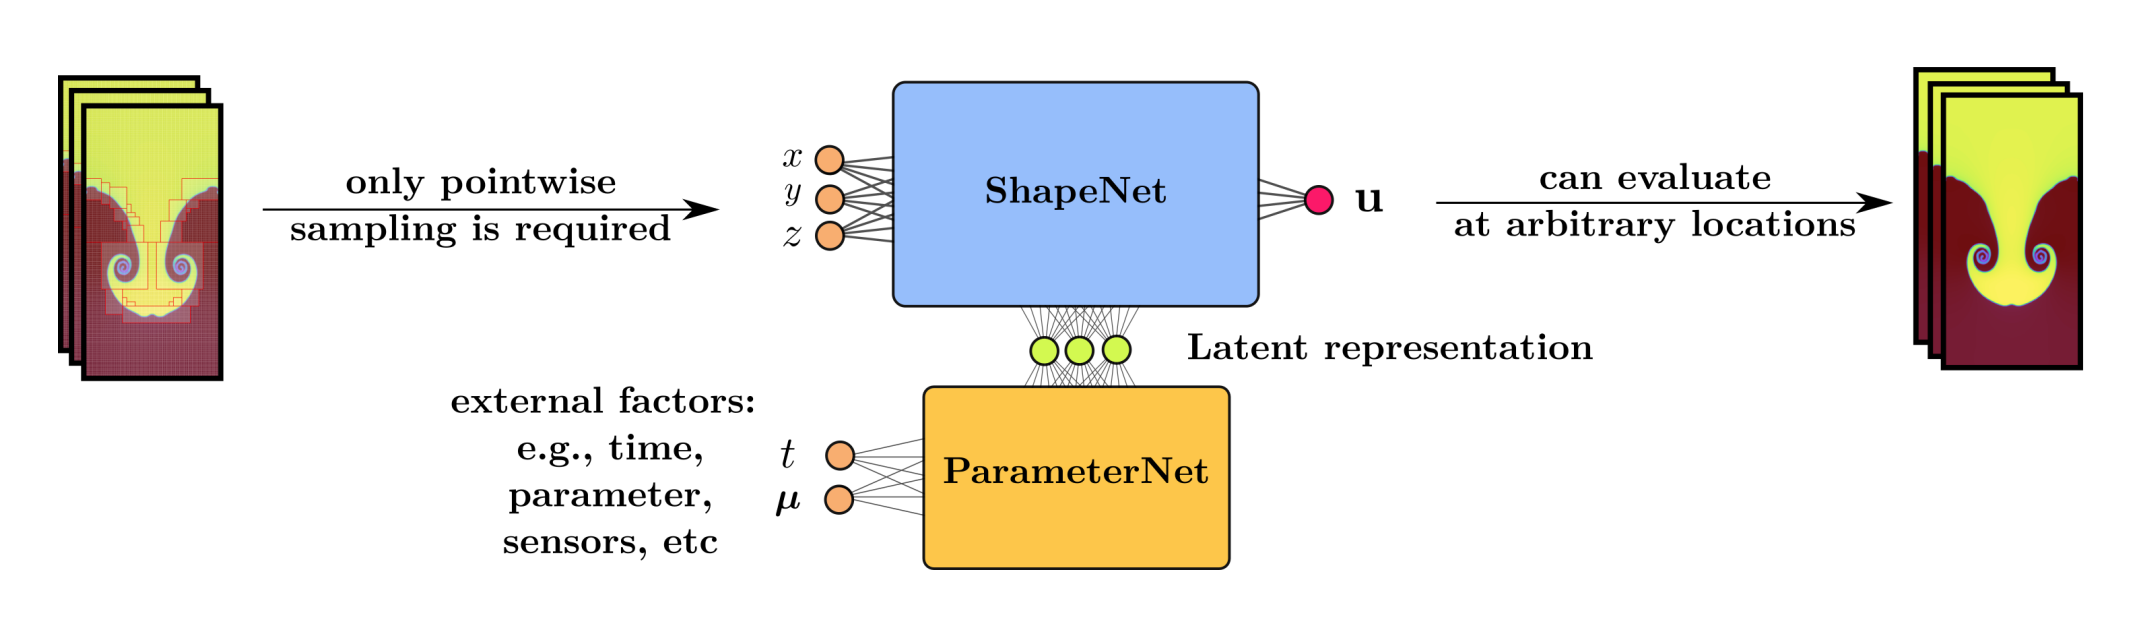
\includegraphics[width=0.7\linewidth]{hypernetwork_diagram.png}
        \caption{NIF Hypernetwork Architecture}
    \end{figure}
\end{frame}

\begin{frame}{Implementation Variants}
    \begin{columns}
        \column{0.5\textwidth}
        \textbf{Upstream \& PyTorch}
        \begin{itemize}
            \item Object-oriented design
            \item Native framework features
            \item Direct tensor operations
        \end{itemize}
        
        \column{0.5\textwidth}
        \textbf{Functional API}
        \begin{itemize}
            \item Functional programming paradigm
            \item Improved composability
            \item Clear data flow
        \end{itemize}
    \end{columns}
\end{frame}

\section{Experimental Setup}
\begin{frame}{Test Cases}
    \begin{columns}
        \column{0.6\textwidth}
        \begin{itemize}
            \item Low frequency wave
            \begin{itemize}
                \item Simple periodic function
                \item Baseline for comparison
            \end{itemize}
            \vspace{2cm}
            \item High frequency complex wave
            \begin{itemize}
                \item Tests model capacity
                \item Challenges interpolation
            \end{itemize}
        \end{itemize}
        
        \column{0.4\textwidth}
        \begin{figure}
            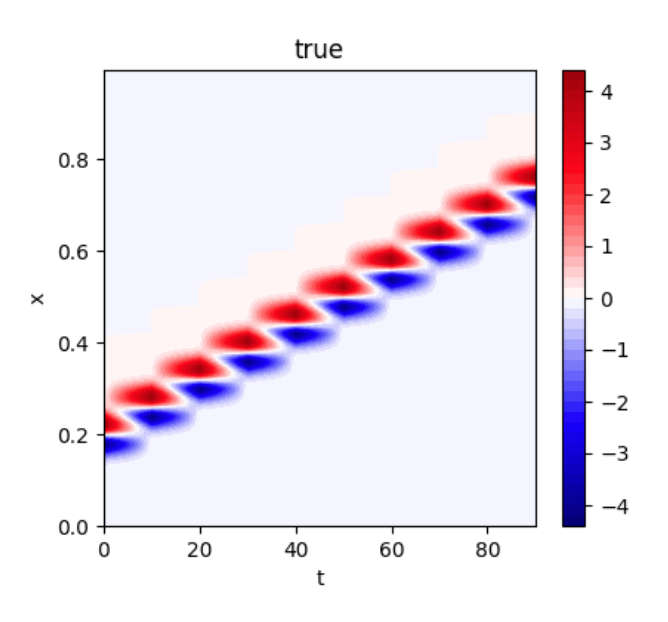
\includegraphics[width=0.5\textwidth]{low_frequency.png}
            \caption*{Low Frequency Wave}
        \end{figure}
        \vspace{0.3cm}
        \begin{figure}
            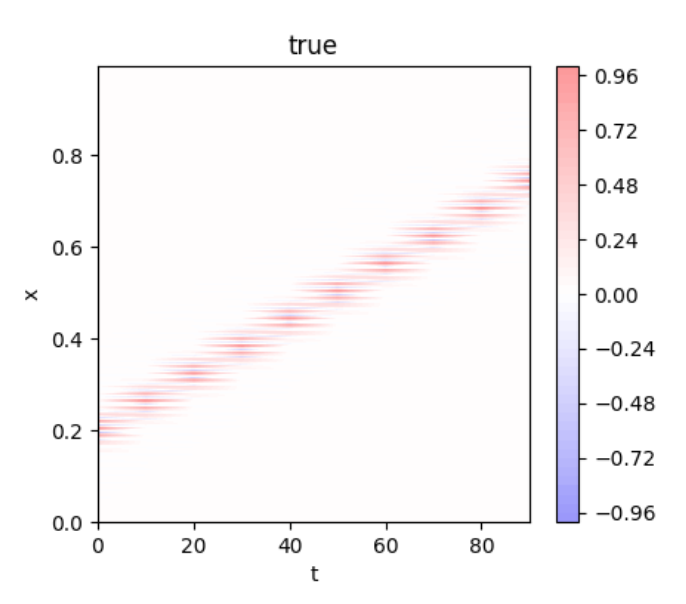
\includegraphics[width=0.5\textwidth]{high_frequency.png}
            \caption*{High Frequency Wave}
        \end{figure}
    \end{columns}
\end{frame}

\begin{frame}{Network Architectures}
    \begin{columns}
        \column{0.5\textwidth}
        \textbf{ShortCut HyperNetwork}
        \begin{itemize}
            \item Direct skip connections
            \item Efficient parameter usage
            \item Faster convergence
        \end{itemize}
        
        \column{0.5\textwidth}
        \textbf{SIREN HyperNetwork}
        \begin{itemize}
            \item Sinusoidal activations
            \item Better frequency fitting
            \item Smooth representations
        \end{itemize}
    \end{columns}
\end{frame}

\section{Results and Analysis}
\begin{frame}{Implementation Results - Upstream}
    \begin{figure}
        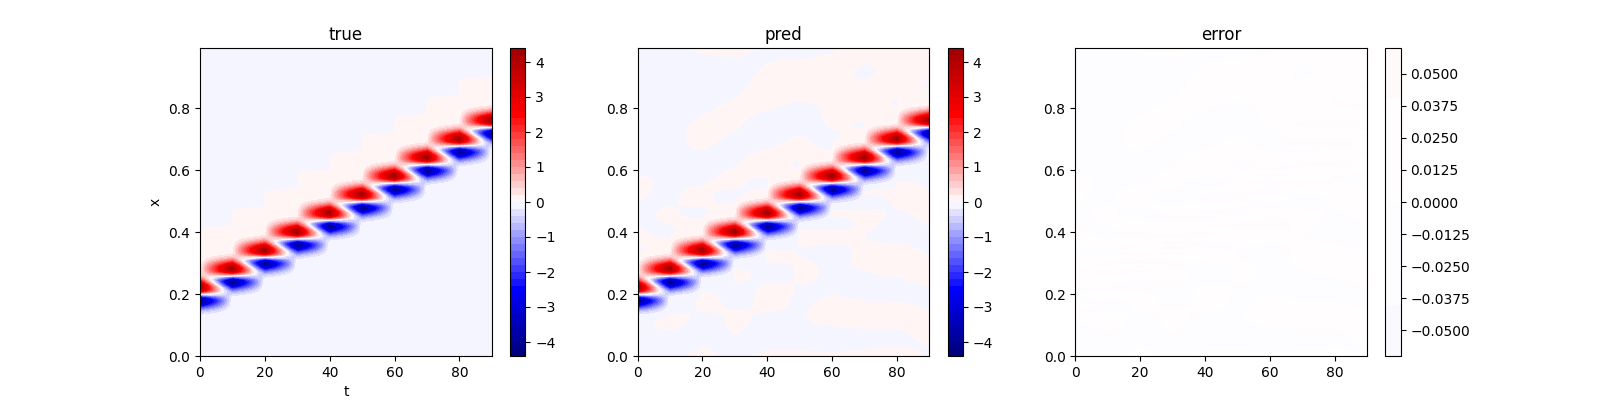
\includegraphics[width=0.95\textwidth]{upstream_vis.png}
        \caption{Upstream Implementation Visualization}
    \end{figure}
    \begin{figure}
        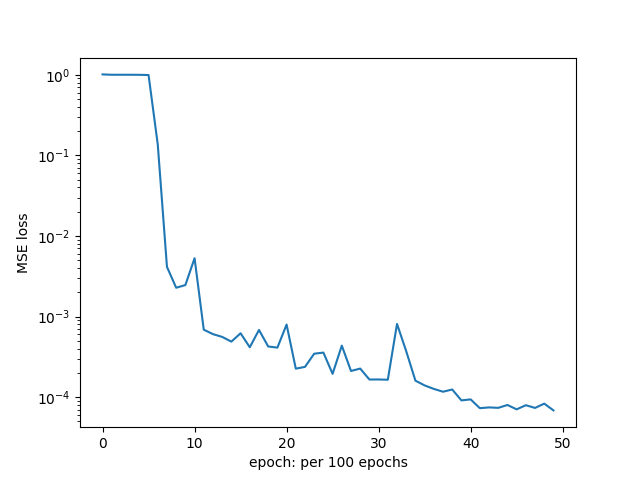
\includegraphics[width=0.3\textwidth]{upstream_loss.png}
        \caption{Upstream Implementation Training Loss}
    \end{figure}
\end{frame}

\begin{frame}{Implementation Results - Functional API}
    \begin{figure}
        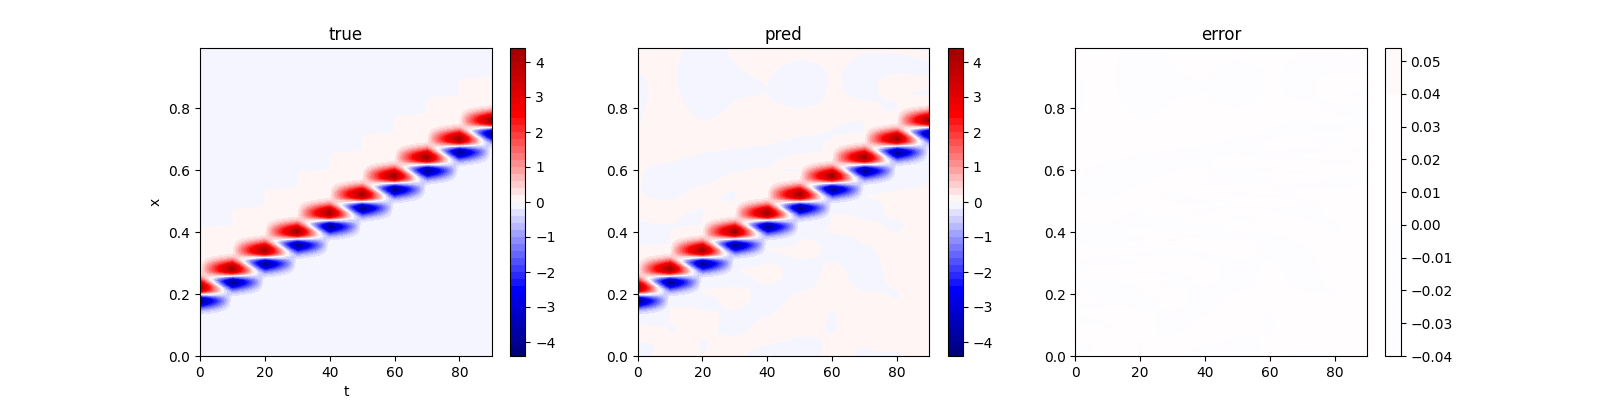
\includegraphics[width=0.95\textwidth]{functional_vis_low.png}
        \caption{Functional API - Low Frequency Wave}
    \end{figure}
    \vspace{0.3cm}
    \begin{figure}
        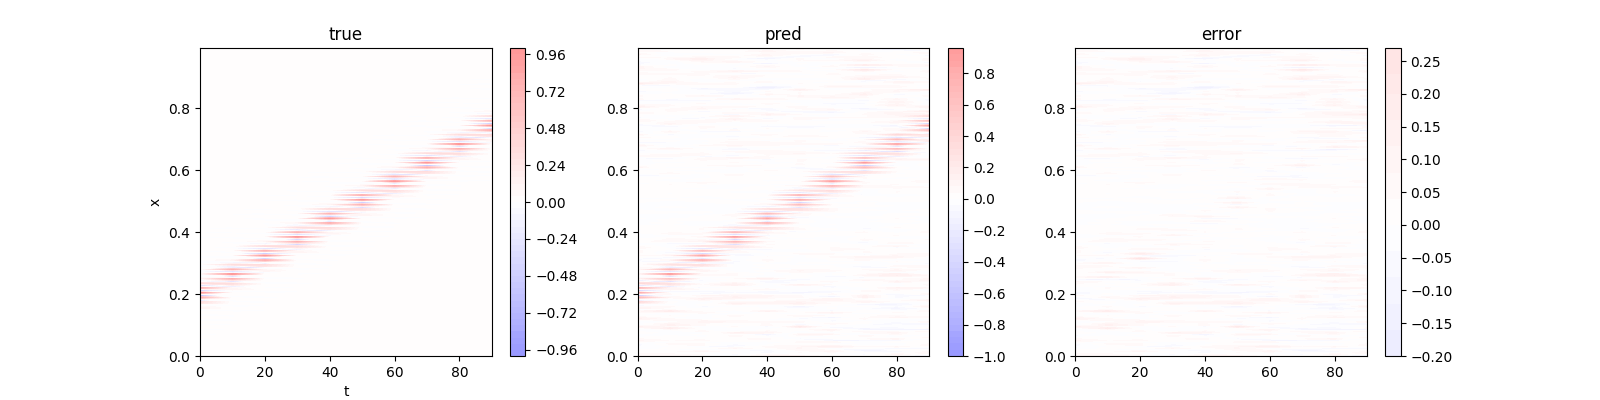
\includegraphics[width=0.95\textwidth]{functional_vis_high.png}
        \caption{Functional API - High Frequency Wave}
    \end{figure}
\end{frame}

\begin{frame}{Training Loss Comparison}
    \begin{figure}
        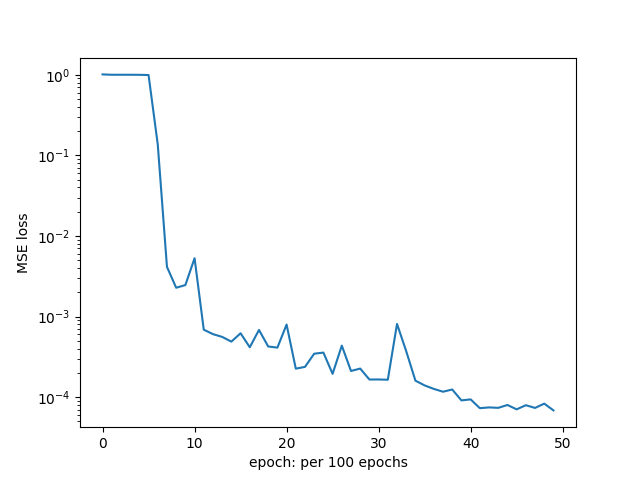
\includegraphics[width=0.32\textwidth]{upstream_loss.png}
        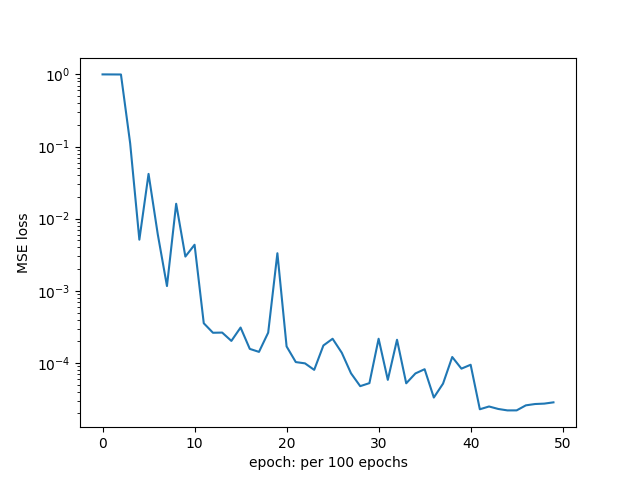
\includegraphics[width=0.32\textwidth]{functional_loss_low.png}
        \caption{Training Loss Comparison (Upstream, Functional API)}
    \end{figure}
    \begin{itemize}
        \item Upstream shows fast convergence (Best loss: 7.316e-05)
        \item Functional API shows 4x better performance (Best loss: 2.198e-05)
    \end{itemize}
\end{frame}

\begin{frame}{Training Loss Comparison}
    \begin{figure}
        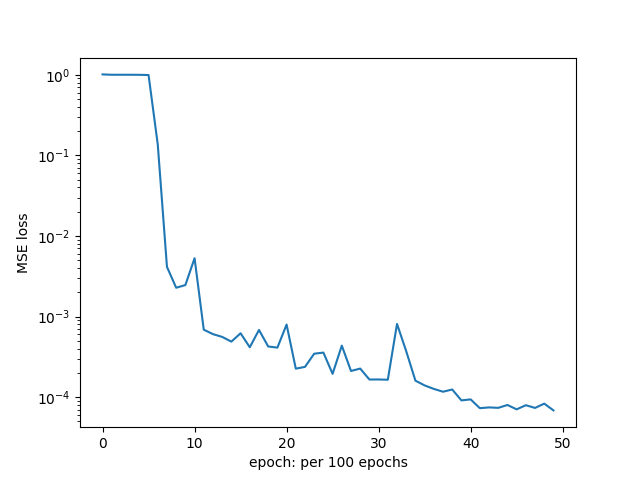
\includegraphics[width=0.32\textwidth]{upstream_loss.png}
        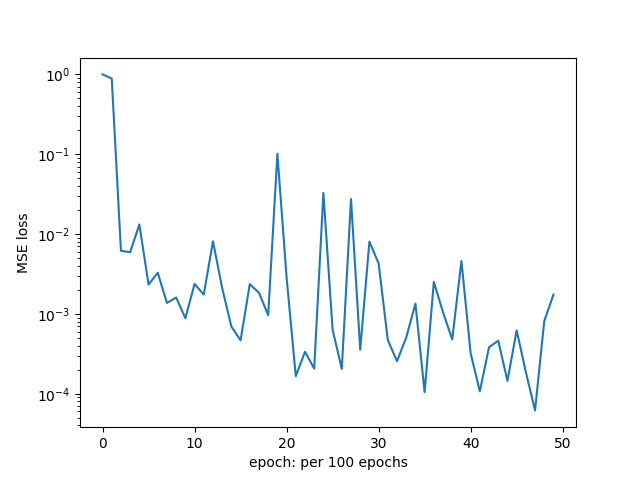
\includegraphics[width=0.32\textwidth]{torch_loss.png}
        \caption{Training Loss Comparison (Upstream, PyTorch)}
    \end{figure}
    \begin{itemize}
        \item Upstream shows fast convergence (Best loss: 7.316e-05)
        \item PyTorch shows similar performance (Best loss: 6.178e-05)
        \item PyTorch shows more variance in performance
    \end{itemize}
\end{frame}

\section{Conclusions}
\begin{frame}{Key Findings \& Future Work}
    \begin{itemize}
        \item Successfully implemented three variants of NIF
        \item Demonstrated effectiveness on both simple cases
        \item Key findings:
        \begin{itemize}
            \item Framework-specific trade-offs
            \item Performance characteristics
            \item Implementation complexity
        \end{itemize}
        \item Future work:
        \begin{itemize}
            \item Additional architectures
            \item More complex test cases
            \item Performance optimizations
        \end{itemize}
    \end{itemize}
\end{frame}

\begin{frame}
    \centering
    \Huge Thank you for your attention!
    
    \vspace{1cm}
    \Large Questions?
\end{frame}

\end{document}
